\part{Integrali Doppi}
\chapter{Integrali Doppi}
\section{Preliminari}
Questo capitolo non è trattato in maniera approfondita poiché:
\begin{description}
	\item[a] tanti e lunghi teoremi fuori contesto per poter introdurre rigorosamente la teoria di Riemann
	\item[b] tale teoria è "superata" da tempo
\end{description}
Il primo è più grosso problema di tale teoria è che non permette il passaggio del limite sotto il segno di integrale, cie\'e per poter scrivere 
$$ \int\lim\limits_{n\to\infty}f_n(x) = \lim\limits_{n\to\infty}\int f_n(x)$$ sono necessarie tante ipotesi molto restrittive.\\
Si è passati cos\'i alla teoria dell'integrale secondo Lebesguw, molto diversa e piuttosto complicata.\\
ESEMPIO...............\\
disegni...........\\
................\\
Il concetto di integrale è quindi molto legato al concetto di area e anche di volume. La teoria di Lebesgue riparte da assiomi come questi definendoli e caratterizzandoli in modo da definire una volta per tutte in maniera sistematica e rigorosa cosa si può e cosa non si può integrare, e dove ha senso parlare di superfici. volumi, ipervolumi, ... 
\section{Regole di Calcolo}
Queste formule permettono di ricondurre il calcolo di integrali doppi a quello di integrali semplici.\\
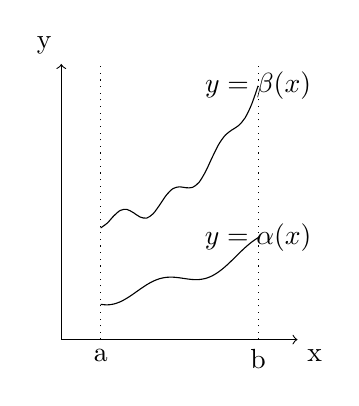
\begin{tikzpicture}
\draw[->] (0,0) -- (3,0) node[anchor=north west] {x};
\draw[->] (0,0) -- (0,3.5) node[anchor=south east] {y};
\draw[dotted] (.5,0) -- (.5,3.5);
\draw[dotted] (2.5,0) -- (2.5,3.5);
\draw (.5,0)  node[anchor=north] {a};
\draw (2.5,0) node[anchor=north] {b};
\draw[domain=.5:2.5,smooth,variable=\x] plot ({\x},{(1/9)*\x*\x*\x+1.5+0.1*sin(10*\x r)}) node {$y=\beta(x)$};
\draw[domain=.5:2.5,smooth,variable=\x] plot ({\x},{(1/9)*\x*\x+0.5+0.1*cos(5*\x r)}) node {$y=\alpha(x)$};
\end{tikzpicture}\\
Se:\\
$a,b\in \R$ con $a<b$\\
$\alpha,\beta\in C^0([a,b];R), \forall x\in[a,b] \alpha(x)\le\beta(x)$\\
$A=\{(x,y)\in \R^2: x\in [a,b] $e$ y\in [\alpha(x),\beta(x)] \}$\\
$f\in C^0(A;R)$\\
Allora\\
$\iint_Af(x,y)dxdy=\int_a^b\left(\int_{\alpha(x)}^{\beta{x}}f(x,y)dy\right)dx$\\
Analogamente.\\
ALTRO GRAFICO....\\
Se:\\
$c,d\in \R$ con $c<d$\\
$\gamma,\delta\in C^0([a,b];R), \forall y\in[c,d] \gamma(y)\le\delta(y)$\\
$A=\{(x,y)\in \R^2: x\in [c,d] $e$ x\in [\gamma(y),\delta(y)] \}$\\
$f\in C^0(A;R)$\\
Allora\\
$\iint_Af(x,y)dxdy=\int_c^d\left(\int_{\gamma(y)}^{\delta{y}}f(x,y)dx\right)dy$
\section{Cambiamento di Variabili}
Se:\\
$A\subseteq \R^2$\\
$\varPhi\in C^1(A;R^2)$
$\varPhi$ è invertibile
$\varPhi^{-1}\in C^1(\varPhi(A);R^2)$\\
$det(D\varPhi)\ne 0$ su $A$\\
$f\in C^0(\varPhi(A);R^2)$\\
Allora:\\
$$ \iint_{\varPhi(A)}f(x,y)dxdy=\iint_A((f\circ g)(u,v))|det(D\varPhi(u,v))|dudv$$
La quantità $det(D\varPhi)$ è spesso chiamato DETERMINANTE JACOBIANO (o semplicemente JACOBIANO) della trasformazione $\varPhi$\\
Adesso spieghiamo perché ild eterminande JACOBIANO, ricordaando A1:
$$ \int_g(A)f(x)dx = \int_Af(g(t))dt$$\\
vari casi\\
...\\
...\\
...\\



